% chktex-file 8

\documentclass[11pt, french]{beamer}

\usepackage{soutenance}

\title{%
  Impact des Fronts sur le Phytoplancton\\
  dans la Région du Gulf Stream\\
  Quantifié par Imagerie Satellitaire
}

\author{Clément Haëck}

\direction{Marina Lévy et Laurent Bopp}

\institute{%
  Laboratoire d'Océanographie et du Climat\\Expérimentations et Analyses Numériques
}

\begin{document}

\begin{frame}[plain, noframenumbering]
  \titlepage%
\end{frame}

%% Préambule
\begin{frame}{Phytoplancton ?}
\end{frame}

\begin{frame}{Problématiques}
\end{frame}

\section{Introduction}

\section{Région subtropicale -- Augmentation de la Chlorophylle dans les fronts}
\begin{frame}
  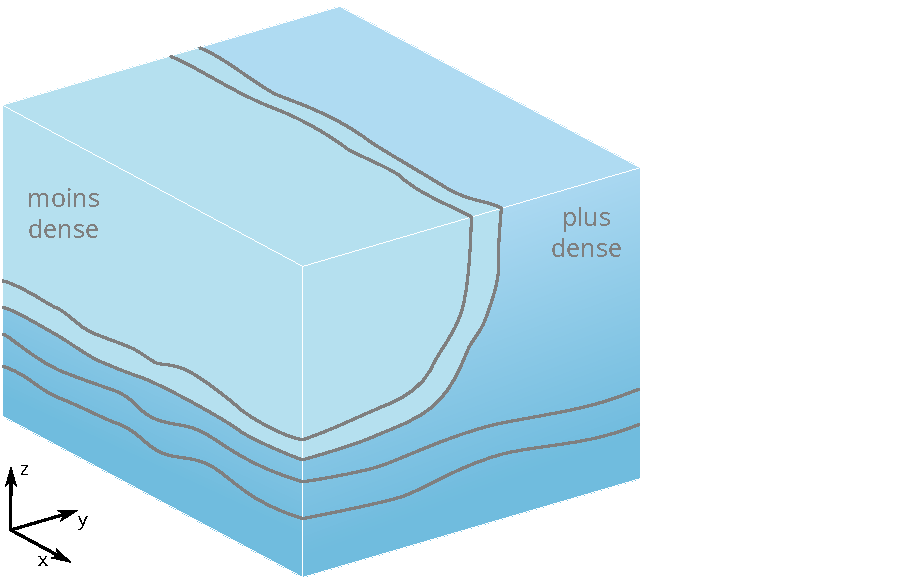
\includegraphics[width=\linewidth]{parts_title/1.pdf}%
\end{frame}

\section{Région du Gulf-Stream -- Intensité des fronts}

\begin{frame}
  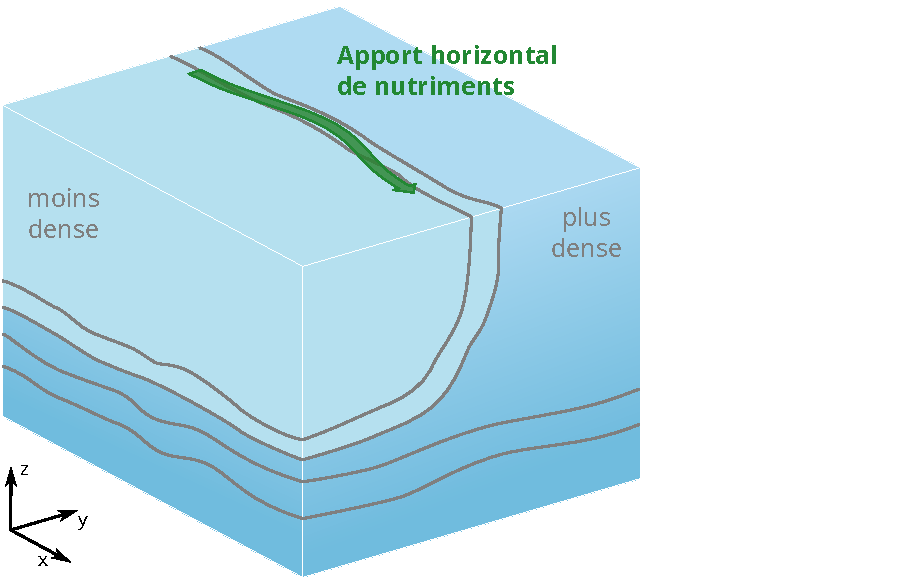
\includegraphics[width=\linewidth]{parts_title/2.pdf}%
\end{frame}

\section{Région subpolaire -- Phénologie du bloom}
\begin{frame}
  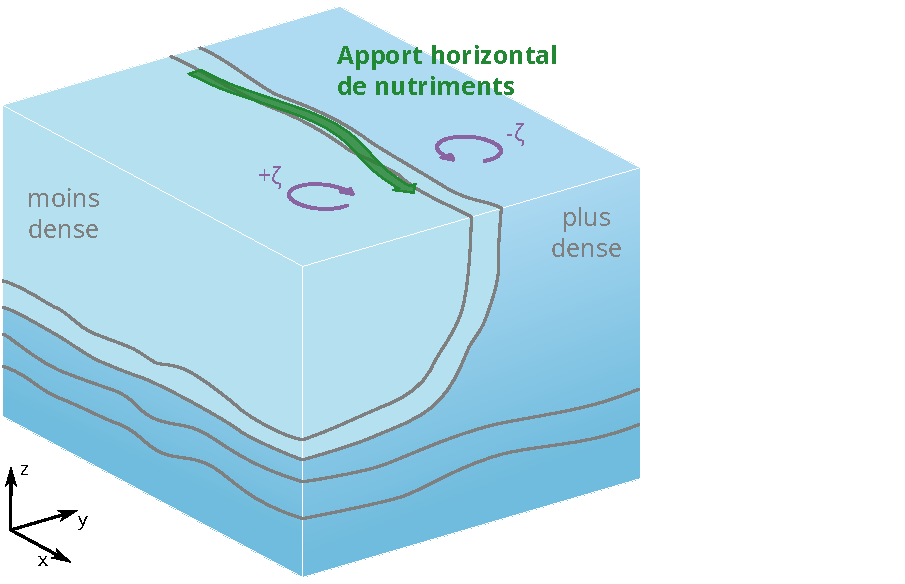
\includegraphics[width=\linewidth]{parts_title/3.pdf}%
\end{frame}

\begin{frame}
\end{frame}

\end{document}
